%% types
\newcommand{\fold}[2]{\let\@tmpop=\relax\@for\@I:=#2\do{\@tmpop\@I\let\@tmpop=#1}}
\newcommand{\record}[1]{\{\fold{,}{#1}\}}
\newcommand{\union}[1]{[\fold{,}{#1}]}
\newcommand{\sq}{\subseteq}

In this section, we describe the parts of the MitM ontology, which is a formal development in the MMT system.
The formalizations can be found at \url{https://gl.mathhub.info/MitM/}.
That location also contains various other archives in the \href{https://gl.mathhub.info/MitM/}{\texttt{MitM} library}, which are experiments, where the MitM ontology has been picked up by other projects.

The MitM ontology consists of two parts: the \textbf{MitM Foundation} which provides the logical language in which the mathematical domains in the MitM ontology can be described, and the \textbf{MitM Core}, which consists of the knowledge about these domains represented in the MitM foundation.

\subsection{The MitM Foundation}\label{sec:foundation}

The MitM foundation provides the type system and logic for the MitM ontology, i.e., the basic representational infrastructure used in the MitM ontology.
It is developed in the archive  \href{https://gl.mathhub.info/MitM/Foundation}{\texttt{Foundation}} (4 files, 539 LoF (lines
of formalization), 103 commits).

\paragraph{Types \& Expressions}
While the logic is relatively straightforward, the standardization of the type system was very difficult because mathematics requires a rich, open-ended type system, yet concrete implementations must stay as simple as possible.
After surveying the OpenDreamKit systems, we developed the types described in Appendix~\ref{app:types}.
These types come with a set of constructors that allow to specify expressions (members of the respective type) that represent mathematical objects systematically; see Appendix~\ref{app:expr} for an exemplary list of mathematical objects that can be represented as a members of these types.

In a nutshell, the MitM foundation provides base types for all arithmetical number systems and common data structures like strings/words and Boolean values.
Complex types build on this include structural ones like (total and partial dependent) function, product, record, types, and mathematical constructions like sets, multisets, ists, vectors, and matrices.
In particular, dependent record types allow to represent types for mathematical structures (e.g. rings, fields, polynomials, finite maps, etc.) and their models.
These can also be constructed from OMDoc/MMT theories via the novel \textsf{Mod} operator~\cite{MueRabKoh:tat18}.

Finally, the MtiM foundation supports subtyping for the arithmetical number systems ($\mathbb{N}\subseteq\mathbb{Z}\subseteq\mathbb{Q}\subseteq\mathbb{R}\subseteq\mathbb{C}$), and along the sub-model relation.
This allows to express many mathematical identies very naturally.


% % % % % % % % % % % % % % % % % % % % % % % % % % % % %
\subsection{MitM Core}

The \textbf{MitM core} in the \href{https://gl.mathhub.info/MitM/smglom}{\texttt{smglom}}\footnote{The name \texttt{smglom} was initially chosen for the ``Semantic Multilingual Glossary of Mathematics'' (SMGloM; see \ref{sec:smglom} below) with which it is cross-referenced. We will rethink naming once the MitM Ontology stabilizes.}  archive (55 files, 2600 LoF, 360 commits).
It carries the bulk of the knowledge representation in the MitM Ontology.
The main thrust of curation has been to get the VRE use cases reported on in~\cite{ODK-D6.5}, but we also have elementary formalizations of algebra, arithmetics, calculus, category theory, set collections, elliptic curves (for LMFDB), functional analysis, geometry, graph theory, measure theory, set theory, and topology.

In the sequel, we describe two exemplary parts of the MitM core ontology.

\subsubsection{Computational Group Theory}
Our formalization of CGT (part of the core ontology, found in \texttt{algebra/computational\_groups}) follows the template of its implementation in \GAP, and requires several levels of abstraction -- currently \emph{abstract}, \emph{representation}, \emph{implementation}, and \emph{concrete}. From our experience, we expect this pattern to be applicable across computational algebra, possibly with additional levels of abstraction. 
The left box in Figure \ref{fig:cgtontology} gives an overview.

The abstract level contains the axioms and basic definitions of the theory of \emph{Groups}: generating sets, homomorphisms, group actions, stabilisers, and orbits.
The most basic part is given in Figure~\ref{fig:mitm1}. 
\begin{figure}[ht]\centering
  \fbox{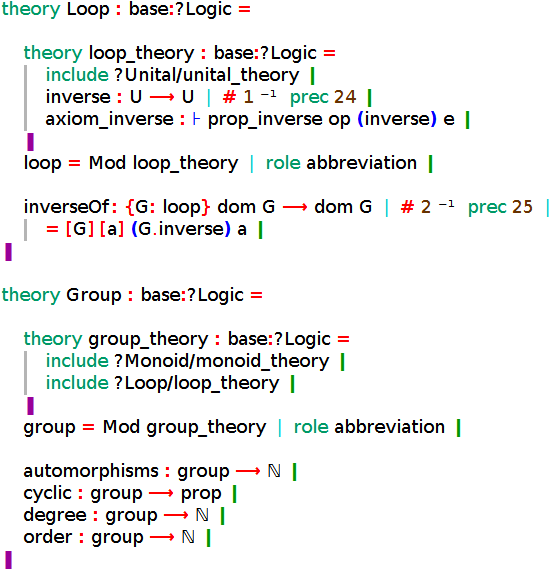
\includegraphics[width=8cm]{groups}}
  \caption{A Formalization of a Group}\label{fig:mitm1}
\end{figure}

At the representation level groups are described as concrete objects
suitable for computations: groups of permutations, groups of matrices,
finitely presented groups, groups obtained by algebraic constructions or using
polycyclic presentations.

At the implementation level, we encode implementation details: for
example, permutation groups are considered as finite subgroups of the group $S_{\mathbb{N}+}$, and constructed by
providing a set of generating permutations.

At the concrete level, the computation happens: while the higher levels
are suitable for mathematical deduction and inference, this level is where OpenDreamKit systems like \GAP perform their main work.

\subsubsection{Modeling and Simulation}

The \href{https://gl.mathhub.info/MitM/smglom}{\texttt{models}}
archive (11 files, 650 LoF, 113 commits) is an experimental extension
of the MitM ontology, where we test the expressive power of MitM
framework (and the OpenDreamKit technologies) by applying it to a
field well outside of mathematics, namely for modeling and simulation
in opto-electronics.

\subsection{The ``Semantic Multilingual Glossary of Mathematics'' (SMGloM)}\label{sec:smglom}

The SMGloM library is available at \url{https://gl.mathhub.info/smglom}. It contains
ca. 815 glossary modules (OMDoc/MMT theories) with more than 1700 concepts. All
represented in \sTeX, a semantic variant of {\LaTeX} developed by FAU and (earlier at)
JacU. Figure~\ref{fig:conductor} shows an example. The boldface words are \emph{definienda}
(i.e. concepts to be defined; here ``conductor'') and the blue ones are concepts already
defined in other parts of the MitM Ontology. SMGloM definitions are multilingual -- mostly
English and German, but also some Romanian, Turkish, Arabic, and Chinese, and are
cross-linked on the concept level.

\begin{figure}[ht]\centering
  \fbox{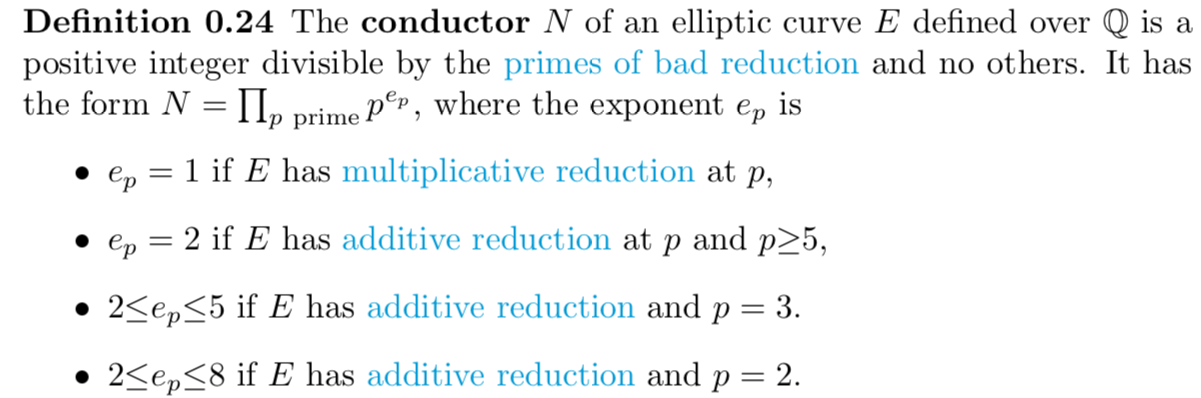
\includegraphics[width=14cm]{conductor}}
  \caption{An \sTeX Definition of the Conductor of an Elliptic
    Curve}\label{fig:conductor}
\end{figure}

The SMGloM library was started in 2013 before the OpenDreamKit project, but only enough content has been developed to fix the data model and system functionality.
About half of the content of the library and all of the informal-formal alignments have been developed in response to needs by OpenDreamKit case studies. 

%%% Local Variables:
%%% mode: visual-line
%%% fill-column: 5000
%%% mode: latex
%%% TeX-master: "report"
%%% End:

%  LocalWords:  formalizations texttt formalization standardization subsubsection textbf newcommand subseteq textsf MueRabKoh:tat18 app:expr
%  LocalWords:  compactitem ednote adic ldots,a_n ldots,a_n ldots,T_n ldots Vec monoid sq
%  LocalWords:  FiniteHybridset subtyping emph leq_T leq_ leq_ leq_ r,x s,y leq doteq_T
%  LocalWords:  t,t forall subformula u,p ldots,x cdot cdot Qsqrt Qzeta th smglom fbox
%  LocalWords:  stabilizes fig:cgtontology fig:mitm1 centering includegraphics mathbb
